\documentclass[10pt,a4paper]{article}
\usepackage[utf8]{inputenc}
\usepackage{amsmath}
\usepackage{amsfonts}
\usepackage{amssymb}
\usepackage{graphicx}
\begin{document}
\begin{center}
\textbf{Universidad de Guayaquil}

\textbf{Facultad de Ciencias Matematicas y Fisicas}

Proyecto de Implantación de un Sistema de Gestión de la Calidad ISO 9001:2015 en el Software SINFIG

\textbf{Integrantes:}

Ramirez Abarca Alex

Ramirez Rios Edinson 

Nicole Navarrete Briones

Curso: SOF-S-MA-3-2
\end{center}
\vspace{\baselineskip}
\textbf{Tabla de Contenido}
\vspace{\baselineskip}

\textbf{1. Normas ISO--------------------------------------------------------------}
\vspace{\baselineskip}

\textbf{2. Caso de Estudio-----------------------------------------------------------}
\vspace{\baselineskip}

\textbf{3. Planificación---------------------------------------------------------------}
\vspace{\baselineskip}

\textbf{4. Código Fuente-------------------------------------------------------------}
\vspace{\baselineskip}

\textbf{5. Conclusión-----------------------------------------------------------------}
\vspace{\baselineskip}

\textbf{1. NORMAS ISO}
\vspace{\baselineskip}

Las normas internacionales hacen que las cosas funcionen. Proporcionan especificaciones de clase mundial para productos, servicios y sistemas, para garantizar la calidad, seguridad y eficiencia. Son fundamentales para facilitar el comercio internacional.
Normas ISO 9001
ISO 9001: 2015 especifica los requisitos para un sistema de gestión de calidad cuando una organización:
a) necesita demostrar su capacidad para proporcionar constantemente productos y servicios que cumplan con los requisitos legales y reglamentarios aplicables del cliente, y
b) tiene como objetivo mejorar la satisfacción del cliente a través de la aplicación efectiva del sistema, incluidos los procesos para la mejora del sistema y el aseguramiento de la conformidad con el cliente y los requisitos legales y reglamentarios aplicables.
Todos los requisitos de ISO 9001: 2015 son genéricos y están destinados a ser aplicables a cualquier organización, independientemente de su tipo o tamaño, o los productos y servicios que proporciona.


\vspace{\baselineskip}
\vspace{\baselineskip}
\textbf{2. CASO DE ESTUDIO}
\vspace{\baselineskip}

Sinfig es un paquete de animación 2D basado en vectores. Está diseñado para ser capaz de producir animaciones con calidad de largometraje. Elimina la necesidad de interpolación, evitando la necesidad de dibujar a mano cada cuadro. Synfig presenta independencia de resolución espacial y temporal (nítida y suave a cualquier resolución o velocidad de fotogramas), imágenes de alto rango dinámico y un sistema de plugin flexible. Synfigstudio es el estudio de animación para synfig y proporciona la GUI interfaz para crear animaciones synfig que se guardan en synfig .sif o formato .sifz.
\vspace{\baselineskip}

\textbf{Características}

\begin{itemize}
\item Produce animaciones de calidad cinematográficas 
\item Mantiene una resolución independiente mente del territorio
\item Tiene una independencia de resolución temporal 
\item Es orientada a un diseño de Artista
\item Las animaciones se trabajan por capas 

\end{itemize}

\textbf{Determinación de los requisitos}
\vspace{\baselineskip}

\textbf{Requisitos Funcionales}
\vspace{\baselineskip}

\begin{itemize}
\item El software producirá animaciones utilizando vectores e ilustraciones de mapas de bits
\item El software deberá tener una amplia paleta de herramientas para mejorar la producción de animaciones
\item El software debe exportar los proyectos en archivos .mp4 
\item El software debe proporcionar mensajes informativos, de ayuda y de error cuando existan 
\item El software debe contener un módulo de ayuda para los usuarios 
\end{itemize}

\textbf{Requisitos No Funcionales}
\vspace{\baselineskip}
\begin{itemize}
\item •	El acceso al software solo debe ser cambiado por el administrador
\item El software debe estar disponibles para plataformas Windows, OS X y Linux
\item El software debe ocupar pocos recursos del sistema
\item El software debe permitir el uso de periféricos de entrada
\end{itemize}

\textbf{Compatibilidad de estándares del mercado}
\vspace{\baselineskip}

ISO 20252



\vspace{\baselineskip}
\vspace{\baselineskip}
\vspace{\baselineskip}
\vspace{\baselineskip}
\vspace{\baselineskip}
\vspace{\baselineskip}


\textbf{Diseño y Desarrollo}
\vspace{\baselineskip}

El software implementa las siguientes interfaces:
\begin{center}
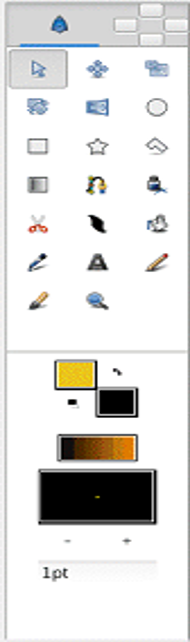
\includegraphics[scale=1]{Imagen1.png}

\textbf{Barra de Herramientas}
\vspace{\baselineskip}

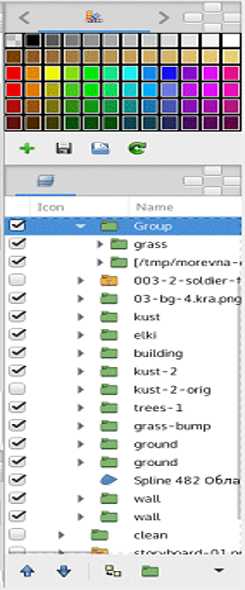
\includegraphics[scale=1]{Imagen2.png}

\textbf{Ventanas de Lienzo-Barra de Navegación}
\vspace{\baselineskip}

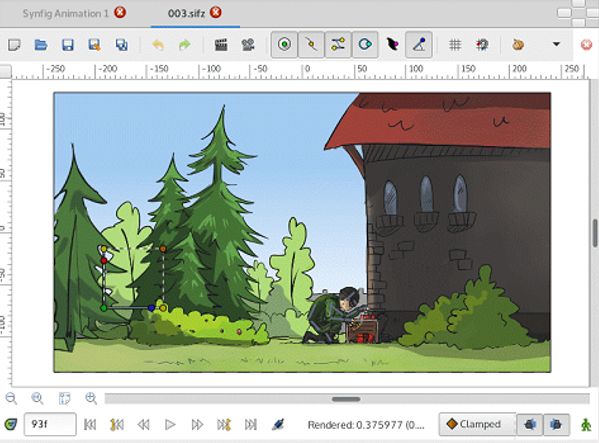
\includegraphics[scale=1]{Imagen3.png}

\textbf{Linea de Tiempo}
\vspace{\baselineskip}
\end{center}

\vspace{\baselineskip}
\vspace{\baselineskip}
\vspace{\baselineskip}
\textbf{3. PLANIFICACIÓN}
\vspace{\baselineskip}

Al planificar el sistema de gestión de la calidad, Synfig. tiene en consideración los riesgos y oportunidades que es necesario abordar con el fin de: 

a) Asegurar que el sistema de gestión de calidad puede lograr los resultados previstos. 

b) Aumentar los efectos deseables. 

c) Prevenir o reducir efectos no deseados.

d) Lograr la mejora.  

\begin{center}
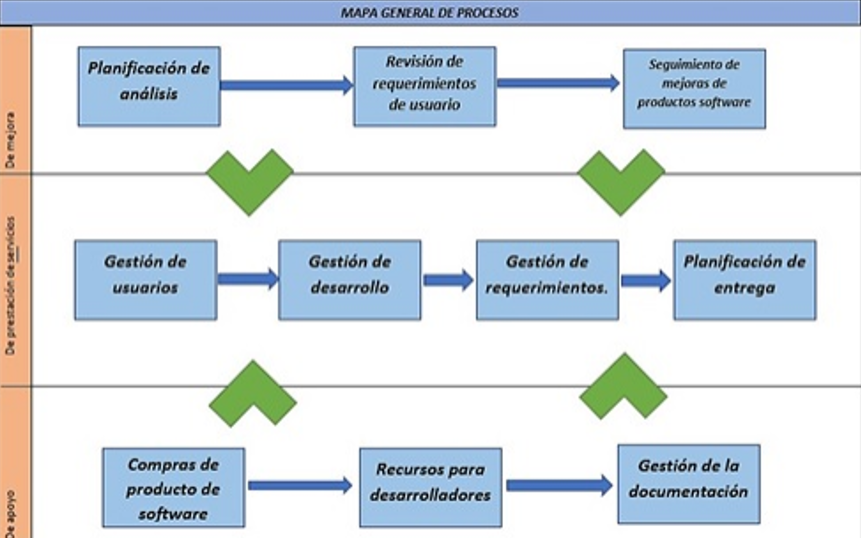
\includegraphics[scale=1]{Imagen4.png}

\textbf{Mapa general de procesos}
\vspace{\baselineskip}
\end{center}


\vspace{\baselineskip}
\textbf{4. CÓDIGO FUENTE}
\vspace{\baselineskip}
\begin{center}
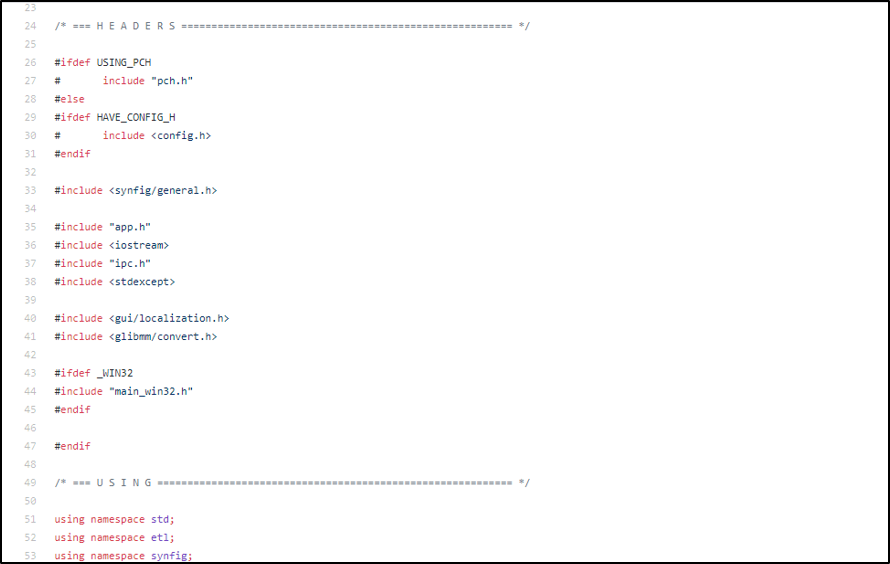
\includegraphics[scale=1]{Imagen5.png}
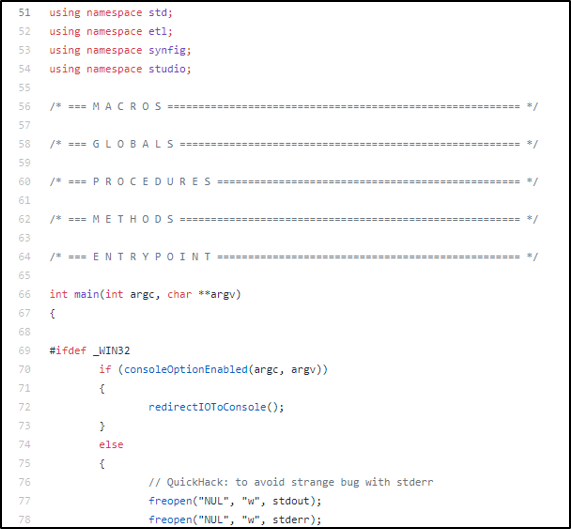
\includegraphics[scale=1]{Imagen6.png}
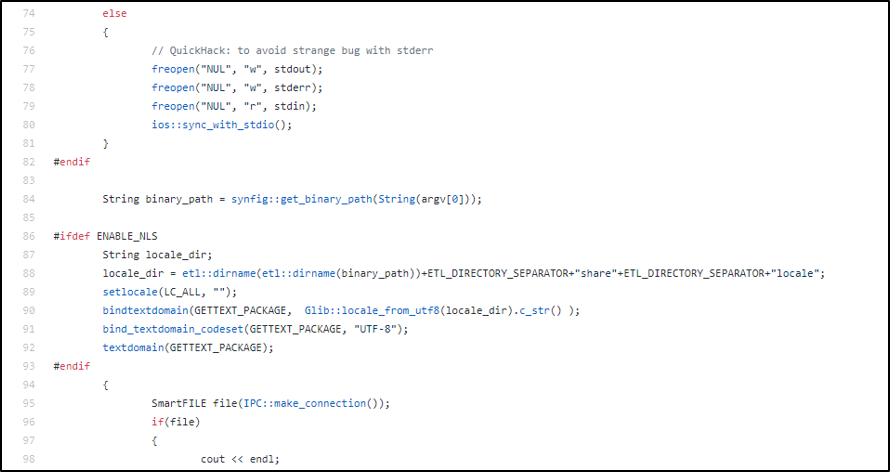
\includegraphics[scale=1]{Imagen8.png}
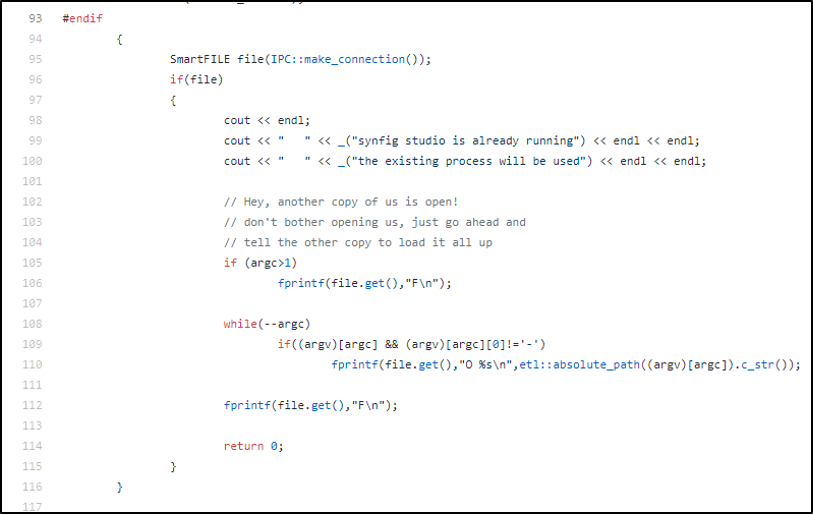
\includegraphics[scale=1]{Imagen9.png}
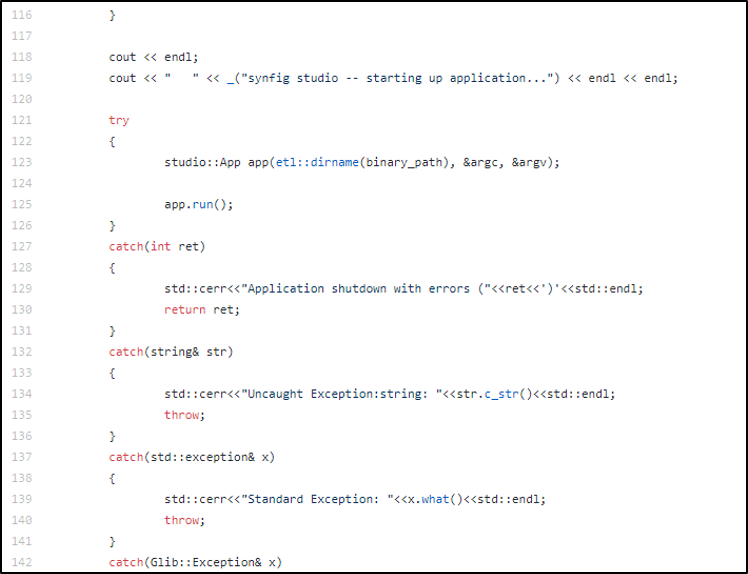
\includegraphics[scale=1]{Imagen10.png}
\end{center}
\vspace{\baselineskip}
\textbf{5. CONCLUSIÓN}
\vspace{\baselineskip}

Podemos concluir que la importancia de implementar un sistema de gestión de la calidad, radica en el hecho de que sirve de plataforma para desarrollar en la organización una serie de actividades, procesos y procedimientos, encaminados a lograr que las características del producto o del servicio cumplan con los requisitos del cliente, que en pocas palabras sean de calidad, lo cual ofrece mayores posibilidades de que sean adquiridos por este, logrando así el porcentaje de ventas planificado por la organización, lo que repercute directamente en los beneficios de todas las partes implicadas.

\vspace{\baselineskip}
\textbf{LINK}

https://github.com/IIIAnthonyIII/Documentacion-Proyecto.git
\end{document}